\documentclass[12pt]{article}
\usepackage[margin=1in]{geometry} 
\usepackage{amsmath,amsthm,amssymb,amsfonts,mathtools}
\usepackage{fancyhdr}
\usepackage{graphicx}
\graphicspath{ {./figures/} }

\newenvironment{problem}[2][]{
    \begin{trivlist}
        \item[
            {\bfseries #1}
            {\bfseries #2}
        ]
}{\end{trivlist}}

\newcommand{\chaptertitle}{Chapter 2 Motion Along A Straight Line}
\newcommand{\sectiontitle}{\textsc{2.5 Freely Falling Bodies}}
\newcommand{\name}{\textsc{Eric Nguyen}}

\pagestyle{fancy}
\chead{\sectiontitle \hfill \textsc{\today} \hfill \name}
\cfoot{\thepage}
\setlength{\headheight}{15pt}

\newcommand{\solution}{\medskip\noindent\textbf{Solution:}}
\newcommand{\Part}[1]{\shortintertext{(#1)}}
\newcommand{\PPart}[1]{\shortintertext{\qquad(#1)}}
\newcommand{\where}{, \, \text{ where }}
\newcommand{\magnitude}[1]{\lVert #1 \rVert}
\newcommand{\Vector}[2]{\langle #1, #2 \rangle}
\newcommand{\UVector}[2]{\left(#1\right)\ihat + \left(#2\right)\jhat}
\newcommand{\ihat}{\hat{\imath}}
\newcommand{\jhat}{\hat{\jmath}}

% UNITS
\newcommand{\unit}[1]{\, \text{#1}}

\newcommand{\cm}{\unit{cm}}
\newcommand{\m}{\unit{m}}
\newcommand{\km}{\unit{km}}
\newcommand{\ft}{\unit{ft}}
\newcommand{\inch}{\unit{in.}}
\newcommand{\mi}{\unit{mi}}
\newcommand{\gcm}{\unit{g/cm}}
\newcommand{\mum}{\, \mu \text{m}}
\newcommand{\mm}{\unit{mm}}

\newcommand{\Liter}{\unit{L}}
\newcommand{\gallon}{\unit{gallon}}
\newcommand{\kg}{\unit{kg}}
\newcommand{\g}{\unit{g}}
\newcommand{\lb}{\unit{lb}}

\newcommand{\mph}{\unit{mi/h}}
\newcommand{\kmh}{\unit{km/h}}
\newcommand{\kms}{\unit{km/s}}
\newcommand{\cms}{\unit{cm/s}}
\newcommand{\mps}{\unit{m/s}}
\newcommand{\mpg}{\unit{mpg}}
\newcommand{\kmL}{\unit{km/L}}

\newcommand{\y}{\unit{y}}
\newcommand{\mo}{\unit{mo}}
\newcommand{\ms}{\unit{ms}}
\newcommand{\ns}{\unit{ns}}
\newcommand{\s}{\unit{s}}
\newcommand{\gs}{\unit{gs}}
\newcommand{\days}{\unit{days}}
\newcommand{\Day}{\unit{day}}
\newcommand{\hours}{\unit{hrs}}
\newcommand{\hour}{\unit{hr}}
\newcommand{\Hour}{\unit{h}}
\newcommand{\minutes}{\unit{mins}}
\newcommand{\minute}{\unit{min}}

\newcommand{\ftpns}{\unit{ft/ns}}
\newcommand{\nspft}{\unit{ns/ft}}

\begin{document}

\begin{problem}{2.35}
    (a) If a flea can jump straight up to a height of 0.440 m, what is its initial speed as it leaves the ground?
    (b) How long is it in the air?

    \solution
    \begin{align}
        \Part{a}
        {v_y}^2 &= {v_{0y}}^2 + 2a_y (y - y_0) \\
        0 &= {v_{0y}}^2 + 2 \left(-9.80 \mps^2\right) \left(0.440 \m\right) \\
        v_{0y} &= \sqrt{2(9.80 \mps^2) (0.440 \m)} \approx 2.94 \mps
        \Part{b}
        y &= y_0 + v_{0y} t + \frac{1}{2} a_y t^2 \\
        0 &= t \left(2.94 \mps + \frac{1}{2} \left(-9.80 \mps^2\right) t\right) \\
        t &= \frac{-2.94 \mps}{-4.90 \mps^2} = 0.600 \s
    \end{align}
\end{problem}

\bigskip

\begin{problem}{2.37}
    A juggler throws a bowling pin straight up with initial speed of 8.20 m/s.
    How much time elapses until the bowling pin returns to the juggler's hand?

    \solution
    \begin{align}
        y &= y_0 + v_{0y} t + \frac{1}{2} a_y t^2 \\
        0 &= t \left(8.20 \mps + \frac{1}{2} \left(-9.80 \mps^2\right) t\right) \\
        t &= \frac{-8.20 \mps}{-4.90 \mps^2} \approx 1.67 \s 
    \end{align}
\end{problem}

\clearpage

\begin{problem}{2.39}
    A tennis ball on Mars, where the acceleration due to gravity is 0.379$g$ and air resistance is negligible, is hit directly upward and returns to the same level 8.5 s later.
    (a) How high above its original point did the ball go?
    (b) How fast was it moving just after it was hit?
    (c) Sketch graphs of the ball's vertical position, vertical velocity, and vertical acceleration as functions of time while it's in the Martian air.

    \solution
    \begin{align}
        \Part{a}
        y &= y_0 + v_{0y} t + \frac{1}{2} a_y t^2 \\
        y &= \frac{1}{2} \left(0.379 \times 9.80 \mps^2\right) \left(\frac{8.5 \s}{2}\right)^2 \approx 33.5 \m
        \Part{b}
        v_y &= v_{0y} + a_y t \\
        0 &= v_{0y} + \left(0.379 \times -9.80 \mps^2\right) \left(\frac{8.5 \s}{2}\right) \\
        v_{0y} &= -\left(0.379 \times -9.80 \mps^2\right) \left(\frac{8.5 \s}{2}\right) \approx 15.8 \mps
        \Part{c}
        y &= \left(15.8 \mps\right) t + \frac{1}{2} \left(0.379 \times -9.80 \mps^2\right) t^2 \\
        v_y &= 15.8 \mps + \left(0.379 \times -9.80 \mps^2\right) t \\
        a_y &= \frac{\left(15.8 \mps + \left(0.379 \times -9.80 \mps^2\right) t\right) - 15.8 \mps}{t} \\
        &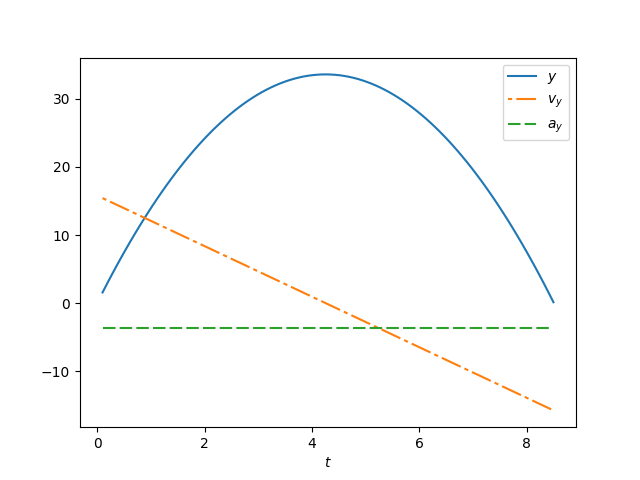
\includegraphics[scale=0.65]{2_39.png}\notag
    \end{align}
\end{problem}

\clearpage

\begin{problem}{2.41}
    \textbf{A Simple Reaction-Time Test.} A meter stick is held vertically above your hand, with the lower end between your thumb and first finger.
    When you see the meter stick released, you grab it with those two fingers.
    You can calculate your reaction time from the distance the meter stick falls, read directly from the point where your fingers grabbed it.
    (a) Derive a relationship for your reaction time in terms of this measured distance, $d$.
    (b) If the measured distance is 17.6 cm, what is your time?

    \solution
    \begin{align}
        \Part{a}
        y &= y_0 + v_{0y} t + \frac{1}{2} a_x t^2 \\
        d &= \frac{1}{2} \left(g\right) t^2 \\
        t &= \sqrt{\frac{2d}{g}}
        \Part{b}
        d &= 17.6 \cm \left(\frac{1 \m}{100 \cm}\right) = 0.176 \m \\
        t &= \sqrt{\frac{2 \left(0.176 \m\right)}{9.80 \mps^2}} \approx 0.190 \s
    \end{align}
\end{problem}

\begin{problem}{2.43}
    \textbf{Launch Failure.} A 7500-kg rocket blasts off vertically from the launch pad with a constant upward acceleration of 2.25 m/s$^2$ and feels no appreciable air resistance.
    When it has reached a height of 525 m, its engines suddenly fail; the only force acting on it is now gravity.
    (a) What is the maximum height this rocket will reach above the launch pad?
    (b) How much time will elapse after engine failure before the rocket comes crashing down to the launch pad, and how fast will it be moving just before it crashes?
    (c) Sketch $a_y$-$t$, $v_y$-$t$, and $y$-$t$ graphs of the rocket's motion from the instant of blast-off to the instant just before it strikes the launch pad.

    \solution
    \begin{align}
        \Part{a}
        t &= \frac{48.6 \mps}{2.25 \mps^2} = 21.6 \s \\
        v_{1y} &= v_{0y} + a_y t = \left(2.25 \mps^2\right) \left(21.6 \s\right) = 48.6 \mps \\
        {v_{2y}}^2 &= {v_{1y}}^2 + 2 a_y \left(y_2 - y_1\right) \\
        0 \mps &= \left(48.6 \mps\right)^2 + 2 \left(-9.80 \mps^2\right) \left(y_2 - 525 \m\right) \\
        y_2 &= \frac{\left(48.6 \mps\right)^2}{2 \left(9.80 \mps^2\right)} + 525 \m \approx 646 \m
    \end{align}
    \begin{align}
        \Part{b}
        y &= y_1 + v_{0y} t + \frac{1}{2} a_y t^2 \\
        0 \m &= 525 \m + \left(48.6 \mps\right) t + \frac{1}{2} \left(-9.80 \mps^2\right) t^2 \\
        t &= \frac{-v_{0y} \pm \sqrt{{v_{0y}}^2 - 4 a_y y_1}}{2 a_y} \\
        &= \frac{-\left(48.6 \mps\right) \pm \sqrt{\left(48.6 \mps\right)^2 - 4 \left(\frac{1}{2} \times -9.80 \mps^2\right) \left(525 \m\right)}}{2 \left(\frac{1}{2} \times -9.80 \mps^2\right)} \\
        &= 16.4 \s \\
        v_{3y} &= v_{1y} + a_y t = -48.6 \mps + \left(9.80 \mps^2\right) \left(16.4 \s\right) \approx 112 \mps 
    \end{align}
    \begin{align*}
        \Part{c}
        y_3 - y_1 &= \frac{1}{2} \left(v_{0y} + v_y\right) t \\
        0 - y_1 &= \frac{1}{2} \left(48.6 \mps + 112 \mps\right) \left(21.6 \s + 16.4 \s\right) \\
        y_1 &= -3051.4 \m \\
        v_{3y} &= v_{1y} + a_y t \\
        112 \mps &= v_{1y} + \left(-9.80 \mps^2\right) \left(16.4 \s\right) \\
        v_{1y} &= 112 \mps + \left(9.80 \mps^2\right) \left(16.4 \s\right) = 272.72 \mps \\
        &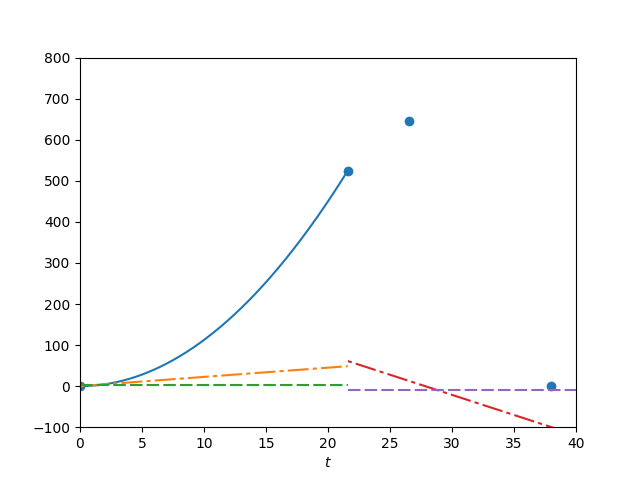
\includegraphics[scale=0.65]{2_43.png}
    \end{align*}
\end{problem}

\clearpage

\begin{problem}{2.45}
    The rocket-driven sled \textit{Sonic Wind No. 2}, used for investigating the physiological effects of large accelerations, runs on a straight, level track 1070 m (3500 ft) long.
    Starting from rest, it can reach a speed of 224 m/s (500 mi/h) in 0.900 s.
    (a) Compute the acceleration in m/s$^2$, assuming that it is constant.
    (b) What is the ratio of this acceleration to that of a freely falling body ($g$)?
    (c) What distance is covered in 0.900 s?
    (d) A magazine article states that at the end of a certain run, the speed of the sled decreased from 283 m/s (632 mi/h) to zero in 1.40 s and that during this time the magnitude of the acceleration was greater than 40$g$.
    Are these figures consistent?

    \solution
    \begin{align}
        \Part{a}
        a_x &= \frac{v_x - v_0}{t} = \frac{224 \mps}{0.900 s} \approx 249 \mps^2 
    \end{align}
    \begin{align}
        \Part{b}
        \frac{249 \mps^2}{9.80 \mps^2} \approx 25.4
    \end{align}
    \begin{align}
        \Part{c}
        x - x_0 &= \frac{1}{2} \left(v_{0x} + v_x\right) t \\
        x - 0 &= \frac{1}{2} \left(0 + 224 \mps\right) \left(0.900 \s\right) \\
        x &\approx 101 \m
    \end{align}
    \begin{align}
        \Part{d}
        a_x &= \frac{v_x - v_0}{t} = \frac{0 - 283 \mps}{1.40 \s} \approx -202 \mps^2 \\
        40g &= 40 \left(9.80 \mps^2\right) = 392 \mps^2 \\
        &\text{No, the figures are not consistent.}
    \end{align}
\end{problem}

\begin{problem}{2.47}
    A 15-kg rock is dropped from rest on the earth and reaches the ground in 1.75 s.
    When it is dropped from the same height on Saturn's satellite Enceladus, the rock reaches the ground in 18.6 s.
    What is the acceleration due to gravity on Enceladus?

    \solution
    \begin{align}
        y &= y_0 + v_{0y} t + \frac{1}{2} a_y t^2 \\
        0 &= y_0 + \frac{1}{2} \left(-9.80 \mps^2\right) \left(1.75 \right)^2 \\
        y_0 &= \frac{1}{2} \left(9.80 \mps^2\right) \left(1.75 \right)^2 \approx 15 \m \\
        0 &= 15 \m + \frac{1}{2} a_y \left(18.6 \s\right)^2 \\
        a_y &= \frac{- 15 \m \cdot 2}{\left(18.6 \s\right)^2} \approx 0.0867 \mps^2
    \end{align}
\end{problem}

\begin{problem}{2.49}
    You throw a small rock straight up from the edge of a highway bridge that crosses a river.
    The rock passes you on its way down, 6.00 s after it was thrown.
    What is the speed of the rock just before it reaches the water 28.0 m below the point where the rock left your hand?
    Ignore air resistance.

    \solution
    \begin{align}
        y &= y_0 + v_{0y} t + \frac{1}{2} a_y t^2 \\
        0 &= 0 + v_{0y} \left(6.00 \s\right) + \frac{1}{2} \left(-9.80 \mps^2\right) \left(6.00 \s\right)^2 \\
        v_{0y} &= \frac{\frac{1}{2} \left(9.80 \mps^2\right) \left(6.00 \s\right)^2}{6.00 \s} = 29.4 \mps \\
        {v_y}^2 &= {v_{0y}}^2 + 2a_y \left(y - y_0\right) \\
        {v_y}^2 &= \left(29.4 \mps\right)^2 + 2 \left(9.80 \mps^2\right) \left(28.0 \m\right) \\
        &= \sqrt{1413.16 \mps} \approx 37.6 \mps
    \end{align}
\end{problem}

\end{document}

